% !TEX encoding   = UTF-8
% !TEX program    = LuaLaTeX
% !TEX spellcheck = de_DE
\documentclass[a4paper]{article}

\usepackage{fontspec}
\usepackage[usenames,dvipsnames]{color}
\usepackage{siunitx}


\usepackage{pgfplots}
\usepackage{pgfplotstable}
\pgfplotsset{compat=newest}
\usepgfplotslibrary{units}


\usepackage{luacode}
\definecolor{skyblue1}{rgb}{0.447,0.624,0.812}
\definecolor{scarletred1}{rgb}{0.937,0.161,0.161}
\definecolor{chameleon1}{rgb}{0.541,0.886,0.204}
%\usepackage{helvet}
\usepackage[landscape]{geometry}
\usepackage{unicode-math}
\usepackage{MnSymbol}
\usepackage[landscape]{geometry}
%\setmainfont{Ubuntu}
%\setmainfont{TeX Gyre Heros}
%\setmathfont{TeX Gyre Heros}
\defaultfontfeatures{Ligatures=TeX}
\newfontfeature{Microtype}{protrusion=default;expansion=default;}
\setmainfont[Microtype,Ligatures=TeX,Numbers=OldStyle]{Minion Pro}
\setsansfont[Microtype,Scale=MatchLowercase,Ligatures=TeX,Numbers=OldStyle]{Myriad Pro}
\renewcommand{\familydefault}{\sfdefault}
\usepackage{fancyhdr}
\pagestyle{fancy}


\rhead{ Gruppe 24}
\setlength{\headheight}{15pt}
\pagenumbering{gobble}
\lhead{Photometrie - \small{Die Extinktionsspektren von $Cu^{2⁺} \rightleftharpoons [Cu \cdot Zincon]^{2 \plus} $ bei Kupferkonzentrationen 0 mg/L, 1 mg/L, 2 mg/L und 4 mg/L -} Anhang 1}
\usetikzlibrary{pgfplots.groupplots}
\begin{luacode*}

local unpack=table.unpack

function drawD()
  local files={}
  local colors={}
  local files = {'iso.csv','iso2.csv','iso3.csv','iso4.csv'}
    local colors = {'blue','orange','red','teal','black','green'}
    local names = {'0 mg/L','1 mg/L','2 mg/L','4 mg/L'}

for filei=1,#files do


    tex.sprint("\\addplot[".."no markers,"..colors[filei].."] coordinates{")


    for line in io.lines(files[filei]) do
           local s, e = line:find("%s+", 1)
            local y=tonumber(line:sub(e))
           local x=tonumber(line:sub(1,e))
        if type(x)  then

        tex.sprint("("..x..","..y..")")

        end
   end

     tex.sprint("};")
              tex.sprint("\\addlegendentry{"..names[filei].."}")

     end

end
function drawE()
  local files={}
  local colors={}
  local files = {'1.TXT','2.TXT','3.TXT','MAX.TXT'}
  --  local files = {'450.TXT','451.TXT','452.TXT','453.TXT','BASELINE.TXT','BASELINE.TXT'}
 local colors = {'blue','orange','red','teal','black','green'}
       local names = {'0 mg/L','1 mg/L','2 mg/L','4 mg/l'}

   -- local shifty = {-0.176238 ,  -0.217737 , -0.211587 ,  -0.182053 , -0.223418,0}
 --local files = {'MAX.TXT'}

for filei=1,#files do

    local wavec = 400
    tex.sprint("\\addplot[".."no markers,"..colors[filei].."] coordinates{")


    for line in io.lines(files[filei]) do
        if type(line)  then
        local coord= line
        --table.insert(lines,line)
        tex.sprint("("..wavec..","..coord..")")
        wavec=wavec+0.853
        end
   end

     tex.sprint("};")
              tex.sprint("\\addlegendentry{"..names[filei].."}")

     end

end


function drawF()
  local files={}
  local colors={}
  local files = {'1A.TXT','2A.TXT','3A.TXT','MAX.TXT'}
  --  local files = {'450.TXT','451.TXT','452.TXT','453.TXT','BASELINE.TXT','BASELINE.TXT'}
 local colors = {'blue','orange','red','teal','black','green'}
       local names = {'0 mg/L','1 mg/L','2 mg/L','4 mg/l'}

   -- local shifty = {-0.176238 ,  -0.217737 , -0.211587 ,  -0.182053 , -0.223418,0}
 --local files = {'MAX.TXT'}

for filei=1,#files do

    local wavec = 400
    tex.sprint("\\addplot[".."no markers,"..colors[filei].."] coordinates{")


    for line in io.lines(files[filei]) do
        if type(line)  then
        local coord= line
        --table.insert(lines,line)
        tex.sprint("("..wavec..","..coord..")")
        wavec=wavec+0.853
        end
   end

     tex.sprint("};")
              tex.sprint("\\addlegendentry{"..names[filei].."}")

     end

end

\end{luacode*}
\newcommand\addplotd{\directlua{drawD()}}
\newcommand\addplote{\directlua{drawE()}}
\newcommand\addplotf{\directlua{drawF()}}

\pgfplotsset{
    standard/.style={
      axis x line=middle,
    axis y line=middle,
     xlabel= Wellenlänge, % Set the labels
    ylabel= Extinktion ,
    x unit= \si{\nano\meter} , % Set the respective units
    y label style={at={(axis description cs:-0.15,.5)},anchor=south,rotate=90},
    x tick label style={rotate=90,anchor=east},
    x label style={at={(axis description cs:0.5,-.13)},anchor=south},
    legend style={draw=none,legend pos=outer north east,legend cell align=left,font=\sffamily},
     minor x tick num={1},
     minor y tick num={1},
     enlargelimits=true,
       xticklabel={$\mathsf{\pgfmathprintnumber{\tick}}$},
    yticklabel={$\mathsf{\pgfmathprintnumber{\tick}}$}
        }
}

\begin{document}

\begin{tabular}{ll}
\begin{tikzpicture}[font=\sffamily]
\begin{axis}[standard,title=Anhand der \textbf{neuen Daten} erstellte Extinktionsspektren]
  \addplotd
\end{axis}
\end{tikzpicture}
&
\begin{tikzpicture}[font=\sffamily]
\begin{axis}[standard,title=Anhand der \textbf{experimentellen} Daten erstellte Extinktionsspektren]
  \addplote
\end{axis}
\end{tikzpicture}
\\
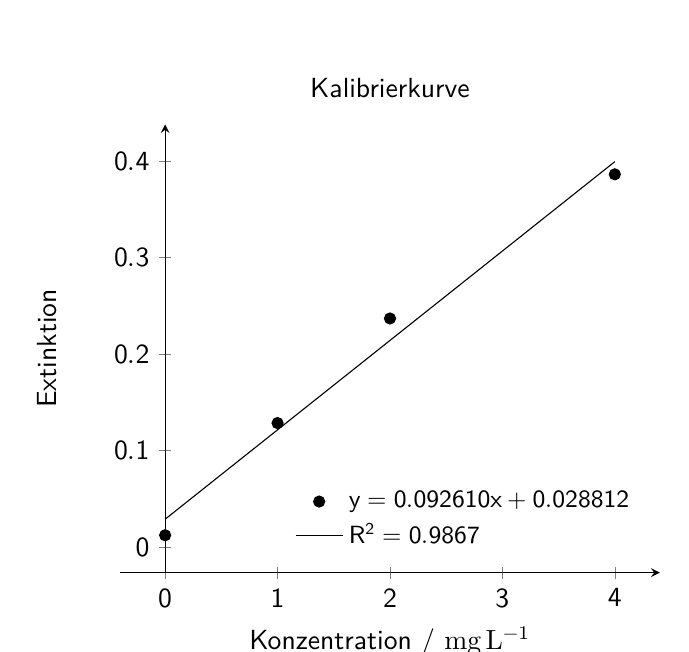
\begin{tikzpicture}[font=\sffamily]
\begin{axis}[axis equal=false,
axis x line=bottom,
axis y line=middle,
legend style={draw=none,legend pos=south east, legend cell align=left, font=\small\sffamily},
xlabel= Konzentration / \si{\milli\gram\per\liter},
ylabel= Extinktion,
y label style={at={(axis description cs:-0.1,.5)},rotate=90,anchor=south},
     enlargelimits=true,
          title= Kalibrierkurve,
            xticklabel={$\mathsf{\pgfmathprintnumber{\tick}}$},
    yticklabel={$\mathsf{\pgfmathprintnumber{\tick}}$}
    ]
\addplot[only marks] table {% plot X versus Y. This is original data.
X Y
0 0.0122
1 0.1284
2 0.23679
4 0.38613
};
\addlegendentry{$\mathsf{y=0.092610x+0.028812}$}
\addplot[domain=0:4] {0.092610*x+0.028812};
\addlegendentry{$\mathsf{R^2=0.9867}$}
\end{axis}
\end{tikzpicture}
&
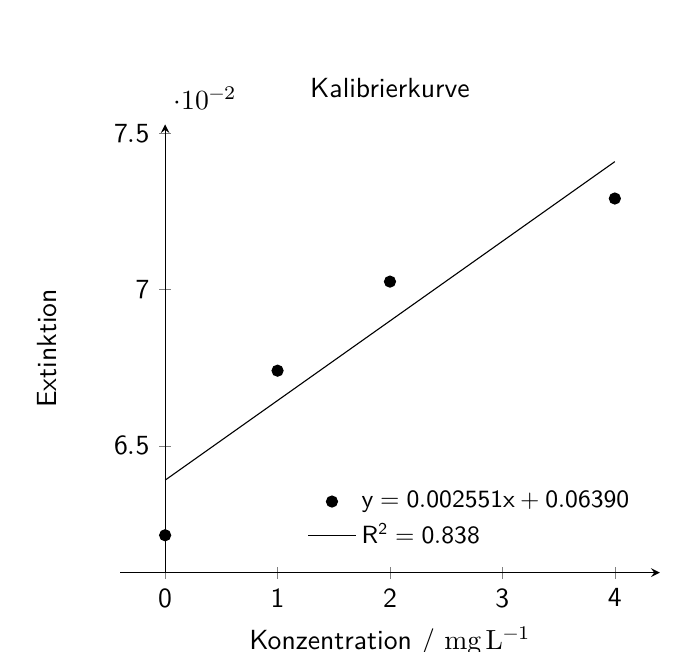
\begin{tikzpicture}[font=\sffamily]
\begin{axis}[axis equal=false,
axis x line=bottom,
axis y line=middle,
legend style={draw=none,legend pos=south east, legend cell align=left,font=\small\sffamily},
xlabel= Konzentration / \si{\milli\gram\per\liter},
ylabel= Extinktion,
y label style={at={(axis description cs:-0.1,.5)},rotate=90,anchor=south},
     enlargelimits=true,
     title= Kalibrierkurve,
       xticklabel={$\mathsf{\pgfmathprintnumber{\tick}}$},
    yticklabel={$\mathsf{\pgfmathprintnumber{\tick}}$}
]
\addplot[only marks] table {% plot X versus Y. This is original data.
X Y
0 0.062135
1 0.067407
2 0.070261
4 0.072923
};
\addlegendentry{$\mathsf{y=0.002551x+0.06390}$}
\addplot[domain=0:4] {0.002551*x+0.06390};
\addlegendentry{$\mathsf{R^2=0.838}$}
\end{axis}
\end{tikzpicture}
\end{tabular}

\par
%\tabellenwerte
\end{document}
